
\documentclass[a4paper,10pt]{article}
\usepackage[utf8]{inputenc}
\usepackage[spanish]{babel}
\usepackage[affil-it]{authblk}
\usepackage{enumerate}
\usepackage{graphicx}
\usepackage{hyperref}
\usepackage{amsmath}
\usepackage{amssymb}
\usepackage{cancel}
\usepackage[usenames, dvipsnames]{color}
\usepackage{tikz}
\usepackage[labelfont=bf]{caption}
\usepackage{subcaption} %Multiple images
\usepackage{multicol} % Multiple columns
\usepackage{float}
\usepackage{cleveref}
 \usepackage{relsize} % bigger math symbols
\usepackage[margin=1.4in]{geometry}
\usepackage[titletoc,toc,title]{appendix}
\usepackage{enumitem}
\usepackage{etoolbox}
\usetikzlibrary{calc}
\numberwithin{equation}{section}

% Circled words
\newcommand{\circled}[2][]{%
  \tikz[baseline=(char.base)]{%
    \node[shape = circle, draw, inner sep = 1pt]
    (char) {\phantom{\ifblank{#1}{#2}{#1}}};%
    \node at (char.center) {\makebox[0pt][c]{#2}};}}
\robustify{\circled}

%Appendices in spanish
\renewcommand{\appendixname}{Ap\'endices}
\renewcommand{\appendixtocname}{Ap\'endices}
\renewcommand{\appendixpagename}{Ap\'endices}

%Zero delimiter
\newcommand{\zerodel}{.\kern-\nulldelimiterspace}

%Columns separation
\setlength{\columnsep}{1cm}

%Indentation
\setlength{\parindent}{0ex}

%Multiple References

\crefrangelabelformat{equation}{(#3#1#4--#5\crefstripprefix{#1}{#2}#6)}

\usepackage{xparse}

%Boxes

\newcommand*{\boxcolor}{blue}
\makeatletter
\renewcommand{\boxed}[1]{\textcolor{\boxcolor}{%
\tikz[baseline={([yshift=-1ex]current bounding box.center)}] \node [rectangle, minimum width=1ex,rounded corners,draw] {\normalcolor\m@th$\displaystyle#1$};}}
 \makeatother

%Constantes
\newcommand{\euler}{\mathrm{e}}
\newcommand{\im}{i}

%Lemas, teoremas, definiciones y pruebas
\newcommand{\definicion}{\textbf{Definición: }}
\newcommand{\lema}{\textbf{Lema: }}
\newcommand{\teorema}{\textbf{Teorema: }}
\newcommand{\prueba}{\textbf{Prueba: }}
\newcommand{\proposicion}{\textbf{Proposición: }}
\newcommand{\corolario}{\textbf{Corolario: }}

% Definición de las secciones y su numeración

\makeatletter
\def\@seccntformat#1{%
  \expandafter\ifx\csname c@#1\endcsname\c@section\else
  \csname the#1\endcsname\quad
  \fi}
\makeatother

%opening
\title{Mecánica Clásica Tarea \# 13}
\author{Favio Vázquez\thanks{Correo: favio.vazquezp@gmail.com}}\affil{Instituto de Ciencias Nucleares. Universidad Nacional Autónoma de México.}
\date{}

\begin{document}

\makeatletter
\def\@maketitle{%
  \newpage
  \null
  \vskip 2em%
  \begin{center}%
  \let \footnote \thanks
    {\Large\bfseries \@title \par}%
    \vskip 1.5em%
    {\normalsize
      \lineskip .5em%
      \begin{tabular}[t]{c}%
        \@author
      \end{tabular}\par}%
    \vskip 1em%
    {\normalsize \@date}%
  \end{center}%
  \par
  \vskip 1.5em}
\makeatother

\maketitle

\section{Problema 1}

Una partícula de masa $m$ se mueve sobre el eje de las $x$ sujeta a un potencial 

$$
V = a\sec^2{\left(\frac{x}{l}\right)},
$$

encuentre la trayectoria por el método de Hamilton-Jacobi.

\vspace{.3cm}

\underline{Solución:} \vspace{.3cm}

Tenemos una partícula que se mueve en sólo una dimensión en el eje $x$, por lo tanto 
podemos escribir la energía cinética como

\begin{equation}
 T = \frac{1}{2}m\dot{x}^2 = \frac{1}{2m}p_x^2,
\end{equation}

y considerando la expresión que tenemos para el potencial, podemos escribir la 
hamiltoniana del sistema como\footnote{Debido a que la lagrangiana $L = T - V$ del 
sistema es independiente del tiempo y la energía cinética es una función cuadrática 
de las velocidades, entonces la cantidad de Jacobi es la energía total del sistema, 
y al escribir a la cantidad de Jacobi en términos de $x$ y $p_x$ tenemos que también 
la hamiltoniana es la energía total del sistema, es decir $H = T+V$.}

\begin{equation}
 H = \frac{1}{2m}p_x^2 + a\sec^2{\left(\frac{x}{l}\right)}.
\end{equation}

Podemos ahora construir la ecuación de Hamilton-Jacobi, que queda expresada como 

\begin{equation}
 \frac{1}{2m}\left(\frac{\partial G}{\partial x}\right)^2 + 
 a\sec^2{\left(\frac{x}{l}\right)} = - \frac{\partial G}{\partial t}.
 \label{eq:HJsec1}
\end{equation}

Claramente esta ecuación se puede resolver por el método de separación de variables,
y proponemos entonces que

\begin{equation}
 G(x,t) = W(x)+ T(t),
\end{equation}

entonces la ecuación \eqref{eq:HJsec1} se convierte en 

\begin{equation}
 \frac{1}{2m}\left(\frac{\partial W}{\partial x}\right)^2 + 
 a\sec^2{\left(\frac{x}{l}\right)} = - \frac{\partial T}{\partial t}.
 \label{eq:HJsec2}
\end{equation}

Debido a que el lado izquierdo de \eqref{eq:HJsec2} depende únicamente de $x$ y el derecho de $t$, el único 
modo de que esta expresión se cumpla es que ambos términos sean iguales a una misma 
constante que llamaremos $\alpha_1$. Entonces,

\begin{equation}
  \frac{1}{2m}\left(\frac{\partial W}{\partial x}\right)^2 + 
 a\sec^2{\left(\frac{x}{l}\right)} = \alpha_1,
\end{equation}

\begin{equation}
 \frac{\partial T}{\partial t} = - \alpha_1.
\end{equation}

De la segunda ecuación vemos que 

\begin{equation}
 T(t) = - \alpha_1t,
\end{equation}

y de la primera ecuación

\begin{equation}
 p_x = \frac{\partial W}{\partial x} = \left\{2m\left[\alpha_1 - a\sec^2{\left(\frac{x}{l}\right)}\right]\right\}^{1/2}.
\end{equation}

y entonces 

\begin{equation}
 W(x) = \int \left\{2m\left[\alpha_1 - a\sec^2{\left(\frac{x}{l}\right)}\right]\right\}^{1/2}dx.
\end{equation}


Por lo tanto tenemos que 

\begin{equation}
 G(x,t) =  \int \left\{2m\left[\alpha_1 - a\sec^2{\left(\frac{x}{l}\right)}\right]\right\}^{1/2}dx
 - \alpha_1t.
\end{equation}

Podemos hallar ahora $\beta_1 = \frac{\partial G}{\partial \alpha_1}$, 

\begin{equation}
 \beta_1 = - t + \int \frac{mdx}{\left\{2m\left[\alpha_1 - a\sec^2{\left(\frac{x}{l}\right)}\right]\right\}^{1/2}}dx.
\end{equation}

De la última ecuación podemos encontrar una ecuación para la trayectoria, $x(t)$, pero 
resulta casi imposible despejar a $x$ de la misma, pero se ha encontrado en términos 
generales la trayectoria del sistema, ya que con encontrar estas expresiones, aunque 
quedan en términos de integrales, se considera resuelto el sistema, esto también 
se da ya que hemos encontrado una expresión para $G$ que contiene toda la información 
del sistema, y obviamente la trayectoria. Para ser completos se muestra debajo el 
resultado de integrar la anterior ecuación, si se desea una expresión 
concreta para $x$ se pueden utilizar algunas aproximaciones o series de potencia.

\begin{equation}
\frac{l\sec{\left(\frac{x}{l}\right)}\sqrt{\alpha_1\cos{\left(\frac{2x}{l}\right)}}
\sqrt{\frac{1}{\alpha_1 - a\sec^2{\left(\frac{x}{l}\right)}}}
\arctan{\left(\frac{\sqrt{2\alpha_1}\sen{\left(\frac{x}{l}\right)}}{\alpha_1\cos{\left(\frac{2x}{l}\right)+ \alpha_1 - 2a}}\right)}}{2\sqrt{\alpha_1}}
= - t - \beta_1
\end{equation}

\section{Problema 2}

Usando los ángulos de Euler como coordenadas, establezca la ecuación de Hamilton-Jacobi 
del trompo simétrico. ¿Se podrá resolver esta ecuación por separación de variables?; 
de ser esto posible encuentre la solución. Puede dejar integrales indicadas.

\vspace{.3cm}

\underline{Solución:} \vspace{.3cm}

En la figura de abajo se muestra un diagrama para trompo simétrico, 

\begin{figure}[H]
 \center 
 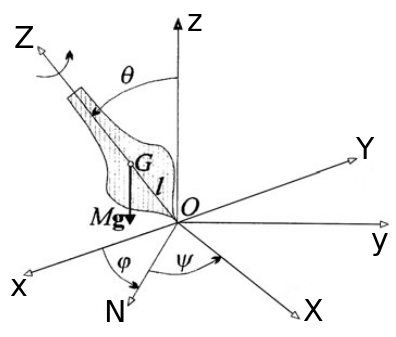
\includegraphics[scale=0.5]{problema2fig1}
 \caption{Trompo simétrico y los ángulos de Euler.}
 \label{fig:problema2fig1}
\end{figure}

Para estudiar el trompo primero tomamos un sistema inercial $(x,y,z)$ cuyo origen 
coincide con el punto fijo y el eje $z$ coincidente con la vertical. Construimos también 
un sistema de referencia $(X,Y,Z)$ anclado al cuerpo con el mismo origen y colocado 
a lo largo de los ejes principales de inercia del trompo, pondremos al eje $Z$ coincidente 
con el eje de simetría. Utilizaremos la convención de denotar las componentes de un 
vector con respecto a los ejes del sistema inercial con letras minúsculas 
y con mayúsculas a las componentes con respecto al sistema anclado al cuerpo. El trompo 
simétrico presenta dos simetrías, una debida a que la fuerza de gravedad 
es siempre vertical, por lo que una rotación en torno a un eje vertical deja invariante 
al sistema y una segunda debida a la simetría propia del trompo. Por esta razón escogemos 
un sistema de coordenadas que contenga a un ángulo de rotación en torno al eje vertical 
y otro en torno al eje del trompo, y este sistema de coordenadas son los conocidos 
ángulos de Euler. En la figura \eqref{fig:problema2fig1} los ángulos de Euler quedan 
definidos en su forma estándar como los ángulos $(\theta,\phi,\psi$). Para no alargar 
más la discusión se asume que ya se conoce lo necesario referente a los ángulos 
de Euler, y que en estas coordenadas el vector de velocidad angular puede descomponerse 
en tres componentes, una de magnitud $\dot{\theta}$ en la dirección de la línea de 
nodos $N$ en \eqref{fig:problema2fig1}, una segunda de magnitud $\dot{\phi}$ en
dirección del eje $z$ y una de magnitud $\dot{\psi}$ en la dirección del eje $Z$. Utilizando 
esto y la figura \eqref{fig:problema2fig1} vemos que las componentes del vector 
velocidad angular pueden obtenerse de estas últimas por medio de 

\begin{align}
 \begin{split}
   \Omega_X &= \dot{\theta}\cos{\psi} + \dot{\phi}\sen{\theta}\sen{\psi}, \\
  \Omega_Y &= - \dot{\theta}\sen{\psi} + \dot{\phi}\sen{\theta}\cos{\psi}, \\
   \Omega_Z &= \dot{\psi} + \dot{\phi}\cos{\theta}.
 \end{split}
\end{align}

La energía cinética puede calcularse fácilmente en las coordenadas del cuerpo, ya que 
el tensor de inercia es constante y diagonal, aparte de que como tratamos con un 
trompo simétrico $I_X = I_Y = I$, y entonces 

\begin{equation}
 T = \frac{1}{2}[I(\Omega_X^2 + \Omega_Y^2) + I_Z\Omega_Z^2],
\end{equation}

\begin{equation}
 \therefore T = \frac{1}{2}\left[I(\dot{\theta}^2 + \dot{\phi}^2\sen^2{\theta})
 + I_Z(\dot{\psi} + \dot{\phi}\cos{\theta})^2\right].
\end{equation}

La única fuerza que interviene es la de la gravedad cuyo potencial es 

\begin{equation}
 V = Mgl\cos{\theta},
\end{equation}

donde $M$ es la masa del trompo, $l$ es la distancia entre el centro de pasas y 
el punto fijo, y $g$ es la aceleración de la gravedad. Entonces la lagrangiana 
$L = T - V$ del trompo simétrico puede escribirse como 

\begin{equation}
 L = \frac{1}{2}\left[I(\dot{\theta}^2 + \dot{\phi}^2\sen^2{\theta})
 + I_Z(\dot{\psi} + \dot{\phi}\cos{\theta})^2\right] - Mgl\cos{\theta}.
\end{equation}

Podemos ver de la lagrangiana que las coordenadas $\phi$ y $\psi$ son ignorables y 
por lo tanto se conservarán sus impulsos asociados. Para 
construir la lagrangiana necesitamos los impulsos generalizados conjugados a las 
coordenadas, que son los siguientes

\begin{align}
 p_\phi &= \dot{\phi}(I\sen^2{\theta} + I_Z\cos^2{\theta}) + I_Z\dot{\psi}\cos{\theta} = \alpha_2, \\
 p_\psi &= I_Z(\dot{\phi}\cos{\theta} + \dot{\psi}) = \alpha_3, \\
 p_\theta &= I\dot{\theta}.
\end{align}

Con un poco de álgebra podemos escribir la hamiltoniana como 

\begin{equation}
 H = \frac{1}{2}\left[\frac{p_\theta^2}{I} + \frac{p_\psi^2}{I_Z} 
 + \frac{(p_\phi - p_\psi\cos{\theta})^2}{I\sen^2{\theta}}\right] + 
 Mgl\cos{\theta}.
\end{equation}

Y la ecuación de Hamilton-Jacobi será entonces 

\begin{equation}
 \frac{1}{2I}\left(\frac{\partial G}{\partial \theta} \right)^2 + 
 \frac{1}{2I\sen^2{\theta}}\left(\frac{\partial G}{\partial \phi} - 
 \frac{\partial G}{\partial \psi}\cos{\theta}\right)^2 + 
 \frac{1}{2I_Z}\left(\frac{\partial G}{\partial \psi} \right)^2 
 + Mgl\cos{\theta} = - \frac{\partial G}{\partial t}.
 \label{eq:HJTrompo1}
\end{equation}

Como la hamiltoniana no depende del tiempo, ni de $\phi$ ni $\psi$ proponemos 
una solución de la forma 

\begin{equation}
 G = \alpha_1t + W(\phi,\theta,\psi) = - \alpha_1t + \alpha_2\phi + \alpha_3\psi 
 + \Theta(\theta).
\end{equation}

Si ahora sustituimos esta expresión en \eqref{eq:HJTrompo1} obtenemos 

\begin{equation}
 \frac{1}{2}\left[\frac{1}{I}\left(\frac{\partial \Theta}{\partial \theta} \right)^2
 + \frac{\alpha_3^2}{I_Z} + \frac{1}{I}\frac{(\alpha_2 - \alpha_3\cos{\theta})^2}{\sen^2{\theta}}\right] 
 + Mgl\cos{\theta} = \alpha_1,
\end{equation}

que como vemos es un ecuación que solo depende de $\theta$ y puede integrarse 
para obtener 

\begin{equation}
 \Theta(\theta) = \int \frac{\sqrt{2I\sen^2{\theta}(\alpha_1 - A - 
 Mgl\cos{\theta}) - (\alpha_2 - \alpha_3\cos{\theta})^2}}{\sen{\theta}}d\theta,
\end{equation}

donde $A = \frac{\alpha_3^2}{2I_Z}$. Por lo tanto la solución para la función que 
contiene toda la información del sistema, $G$, es 

\begin{equation*}
 \boxed{G = -\alpha_1t + \alpha_2\phi + \alpha_3\psi + \int \frac{\sqrt{2I\sen^2{\theta}(\alpha_1 - A - 
 Mgl\cos{\theta}) - (\alpha_2 - \alpha_3\cos{\theta})^2}}{\sen{\theta}}d\theta.}
\end{equation*}

Ahora solo nos falta calcular las $\beta^i$ y los impulsos utilizando la formulación 
de Hamilton-Jacobi. Entonces 

\begin{equation}
 \beta^1 = \frac{\partial G}{\partial \alpha_1} = 
 - t + \int \frac{I\sen{\theta}}{\sqrt{2I\sen^2{\theta}(\alpha_1 - A - 
 Mgl\cos{\theta}) - (\alpha_2 - \alpha_3\cos{\theta})^2}}d\theta,
\end{equation}

\begin{equation}
 \beta^2 = \frac{\partial G}{\partial \alpha_2} = 
 \phi + \int \frac{\csc{\theta}(\alpha_2 - \alpha_3\cos{\theta})}{\sqrt{2I\sen^2{\theta}(\alpha_1 - A - 
 Mgl\cos{\theta}) - (\alpha_2 - \alpha_3\cos{\theta})^2}}d\theta,
\end{equation}

\begin{equation}
 \beta^3 = \frac{\partial G}{\partial \alpha_3} = 
 \psi + \int \frac{\cot{\theta}(\alpha_2 - \alpha_3\cos{\theta})}{\sqrt{2I\sen^2{\theta}(\alpha_1 - A - 
 Mgl\cos{\theta}) - (\alpha_2 - \alpha_3\cos{\theta})^2}}d\theta.
\end{equation}

Por último expresamos los impulsos,

\begin{equation}
 p_\theta = \frac{\partial G}{\partial \theta} = 
 \frac{\sqrt{2I\sen^2{\theta}(\alpha_1 - A - 
 Mgl\cos{\theta}) - (\alpha_2 - \alpha_3\cos{\theta})^2}}{\sen{\theta}},
\end{equation}

\begin{equation}
 p_\phi = \frac{\partial G}{\partial \psi} = \alpha_2,
\end{equation}

\begin{equation}
 p_\psi = \frac{\partial G}{\partial \psi} = \alpha_3.
\end{equation}

Con lo cual vemos un significado directo para $\alpha_2$ y $\alpha_3$, que ya lo sabíamos 
de antemano pero quisimos probarlo al final. Puede verse fácilmente entonces viendo 
estas ecuaciones que $\alpha_1$ será la energía total del trompo simétrico. Con esto
hemos demostrado que el problema del trompo simétrico utilizando los ángulos 
de Euler como coordenadas generalizadas, se puede resolver por separación 
de variables y hemos encontrado una solución completa al mismo.

\section{Problema 3}

Demuestra que la ecuación de Hamilton-Jacobi de una partícula atraída por dos centros
gravitatorios iguales que se encuentran a una distancia fija $l$ es separable en coordenadas 
elípticas confocales. 

\vspace{.3cm}

\underline{Solución:} \vspace{.3cm}

\textbf{Nota: El profesor nos dijo que podíamos resolver el problema en dos dimensiones.}

\vspace{.3cm}

\textbf{Notación: Cambiaremos $l$ por $a$ debido a que es más fácil de distinguir tanto 
para las imágenes como para las ecuaciones.}

\vspace{.3cm}

Las coordenadas elípticas confocales $u$ y $v$ están relacionadas con las coordenadas 
cartesianas $(x,y)$ por 

\begin{align}
 x = a\cosh{u}\cos{v}, \\
 y = a\senh{u}\sen{v}.
\end{align}

Los rangos de $u$ y $v$ son $0 \leq u < \infty$ y $0 \leq v < 2\pi$. Para encontrar
las curvas coordenadas primero hacemos $u$ constante, y tenemos que 

\begin{equation}
 \frac{x^2}{\cosh^2{u}} + \frac{y^2}{\senh^2{u}} = a^2,
 \label{eq:uelipse}
\end{equation}

y llamando a $A = \cosh{u}$ y $B = \senh{u}$ tenemos 

\begin{equation}
 \frac{x^2}{A^2} + \frac{y^2}{B^2} = a^2,
\end{equation}

y vemos claramente que las curvas de $u$ constante son elipses. Ahora consideremos 
a $v$ constante, tenemos que 

\begin{equation}
 \frac{x^2}{\cos^2{v}} - \frac{y^2}{\sen^2{v}} = a^2,
 \label{eq:vhiperbola}
\end{equation}

y llamando a $C = \cos{v}$ y $D = \sen{v}$ tenemos 

\begin{equation}
 \frac{x^2}{C^2} - \frac{y^2}{D^2} = a^2,
\end{equation}

y vemos que cada curva de $v$ constante es una hipérbola que se abre en las direcciones 
de $\pm x$. Puede probarse \cite{arfken} que todas estas curvas tienen los mismos focos en $y=0$, 
$x= \pm a$ y que las elipses intersectan a las hipérbolas en ángulos rectos. Debajo se encuentra 
una representación gráfica de estas coordenadas con los resultados que hemos obtenido.

\begin{figure}[H]
 \center 
 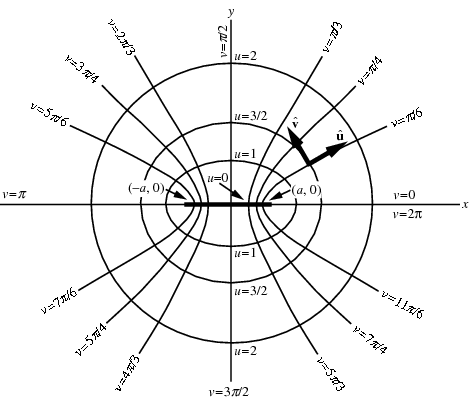
\includegraphics[scale=0.7]{problema3fig1}
 \caption{Coordenadas confocales elípticas $(u,v)$ en el plano. Las curvas de 
 $u$ constante son elipses y las de $v$ constante son hipérbolas.}
 \label{fig:problema3fig1}
\end{figure}

Para resolver este problema fijaremos los focos de las coordenadas elípticas en los 
centros gravitatorios fijos $(x,y) = (\pm a,0)$, ver figura \eqref{fig:problema3fig1}. La hamiltoniana es entonces 

\begin{equation}
 H = \frac{p^2}{2m} + V(r_1,r_2),
\end{equation}

donde el potencial $V$ depende de las distancias $r_1$ y $r_2$ hacia los dos 
centros de fuerza y está dado por 

\begin{equation}
 V(r_1,r_2) = - \left(\frac{\alpha_1}{r_1} + \frac{\alpha_2}{r_2} \right)
  = \left(\frac{\alpha_1}{(x - a)^2 + y^2} + \frac{\alpha_2}{(x + a)^2 + y^2}\right),
\end{equation}

donde las $\alpha_i$ son las fuerzas de los centros de fuerza. Ahora reescribiremos 
$H$ en términos de $(u,v)$, para eso utilizamos el hecho de podemos escribir al potencial 
en términos de $(u,v)$ como (utilizando \eqref{eq:uelipse} y \eqref{eq:vhiperbola})

\begin{equation}
 V(u,v) = - \frac{\alpha \cosh{u} - \alpha'\cos{v}}{\cosh^2{u}- \cos^2{v}},
\end{equation}

donde $alpha \equiv \alpha_1 + \alpha_2$ y $\alpha' \equiv \alpha_1 - \alpha_2$. Y ahora 
reescribiremos la energía cinética en términos de los impulsos conjugados 

\begin{equation}
 p_u = \frac{\partial L}{\partial \dot{u}} = \frac{\partial T}{\partial \dot{u}},
\end{equation}

\begin{equation}
 p_v = \frac{\partial L}{\partial \dot{v}} = \frac{\partial T}{\partial \dot{v}},
\end{equation}

debido a que $V$ es independiente de $\dot{u}$ y $\dot{v}$. Entonces 

\begin{equation}
 T = \frac{1}{2} (\dot{x}^2 + \dot{y}^2) = \frac{1}{2}a^2m(\cosh^2{u} - \cos^2{v})
 (\dot{u}^2+\dot{v}^2),
\end{equation}

por lo tanto

\begin{equation}
 p_u = a^2m(\cosh^2{u} - \cos^2{v})\dot{u},
\end{equation}

y 

\begin{equation}
 p_v = a^2m(\cosh^2{u} - \cos^2{v})\dot{v},
\end{equation}

y encontramos ahora una expresión para $\dot{u}$ y $\dot{v}$ en términos de 
$p_u$ y $p_v$, 

\begin{equation}
 \dot{u} = \frac{p_u}{a^2m(\cosh^2{u} - \cos^2{v})}
\end{equation}

y 

\begin{equation}
 \dot{v} = \frac{p_v}{a^2m(\cosh^2{u} - \cos^2{v})}
\end{equation}

y entonces 

\begin{equation}
 T = \frac{1}{2}a^2m(\cosh^2{u} - \cos^2{v})\left( \frac{p_u^2}{a^4m^2(\cosh^2{u} - \cos^2{v})^2} 
 + \frac{p_v^2}{a^4m^2(\cosh^2{u} - \cos^2{v})^2}\right).
\end{equation}

\begin{equation}
 \therefore T = \frac{1}{2}\left( \frac{p_u^2 + p_v^2}{a^2m(\cosh^2{u} - \cos^2{v})}\right).
\end{equation}


Podemos ahora escribir la hamiltoniana en estas nuevas coordenadas como 

\begin{equation}
 H = T + V = \frac{1}{2a^2m}\left( \frac{p_u^2 + p_v^2}{\cosh^2{u} - \cos^2{v}}\right) - \frac{\alpha \cosh{u} - \alpha'\cos{v}}{\cosh^2{u}- \cos^2{v}},
\end{equation}

\begin{equation}
 \therefore H = \frac{1}{2a^2m}\left( \frac{p_u^2 + p_v^2 - 2a^2m\alpha \cosh{u} + 2a^2m\alpha'\cos{v}}{\cosh^2{u}- \cos^2{v}}\right)
\end{equation}

Ahora escribimos la ecuación de Hamilton-Jacobi como

\begin{equation}
\frac{1}{2a^2m}\left( \frac{\left(\frac{\partial G}{\partial u} \right)^2 + 
\left(\frac{\partial G}{\partial v} \right)^2- 2a^2m\alpha \cosh{u} + 
2a^2m\alpha'\cos{v}}{\cosh^2{u}- \cos^2{v}}\right) = - \frac{\partial G}{\partial t}.
\label{eq:HJconfocales1}
\end{equation}

Para comprobar si esta ecuación en derivadas parciales es soluble por el método de 
separación de variables proponemos una solución del estilo 

\begin{equation}
 G(u,v,t) = W(u,v) + T(t),
\end{equation}

y entonces la ecuación \eqref{eq:HJconfocales1} se transforma en 

 \begin{equation}
\frac{1}{2a^2m}\left( \frac{\left(\frac{\partial W}{\partial u} \right)^2 + 
\left(\frac{\partial W}{\partial v} \right)^2- 2a^2m\alpha \cosh{u} + 
2a^2m\alpha'\cos{v}}{\cosh^2{u}- \cos^2{v}}\right) = - \frac{\partial T}{\partial t}.
\label{eq:HJconfocales2}
\end{equation}

Vemos que el único modo de que se cumpla la igualdad \eqref{eq:HJconfocales2} es que 
ambos lados sean iguales a una constante que llamaremos $\zeta_1$, y tenemos entonces 

\begin{equation}
 \frac{1}{2a^2m}\left( \frac{\left(\frac{\partial W}{\partial u} \right)^2 + 
\left(\frac{\partial W}{\partial v} \right)^2- 2a^2m\alpha \cosh{u} + 
2a^2m\alpha'\cos{v}}{\cosh^2{u}- \cos^2{v}}\right) = \zeta_1,
\end{equation}

\begin{equation}
 \frac{\partial T}{\partial t} = - \zeta_1.
\end{equation}

De la segunda de estas ecuaciones vemos que 

\begin{equation}
 \boxed{T(t) = - \zeta_1t,}
\end{equation}

y la primera la podemos reescribir como 

\begin{equation}
\left(\frac{\partial W}{\partial u} \right)^2 + 
\left(\frac{\partial W}{\partial v} \right)^2
= 2a^2m\zeta_1(\cosh^2{u}- \cos^2{v})
+ 2a^2m\alpha \cosh{u} - 
2a^2m\alpha'\cos{v}.
\end{equation}

Ya hemos separado la parte temporal, ahora proponemos una solución del tipo 

\begin{equation}
 W(u,v) = W_u(u) + W_v(v),
\end{equation}

y entonces tenemos que 

\begin{equation}
\left(\frac{\partial W_u}{\partial u} \right)^2 + 
\left(\frac{\partial W_v}{\partial v} \right)^2
= 2a^2m\zeta_1(\cosh^2{u}- \cos^2{v})
+ 2a^2m\alpha \cosh{u} - 
2a^2m\alpha'\cos{v},
\end{equation}

reescribiendo vemos que 

\begin{equation}
 \left(\frac{\partial W_u}{\partial u} \right)^2 - 2a^2m\zeta_1\cosh^2{u} - 
 2a^2m\alpha\cosh{u} = 
 - \left(\frac{\partial W_v}{\partial v} \right)^2 - 2a^2m\zeta_1\cos^2{v} - 
 2a^2m\alpha'\cos{v}.
 \label{eq:HJconfocales3}
\end{equation}

Como vemos el lado izquierdo de \eqref{eq:HJconfocales3} solo depende de $u$ y 
el lado derecho de $v$ por lo tanto el único como de que se mantenga esta igualdad 
es que ambos lados sean iguales a una misma constante que llamaremos $\zeta_2$, 
y entonces 

\begin{equation}
 \boxed{\left(\frac{\partial W_u}{\partial u} \right)^2 - 2a^2m\zeta_1\cosh^2{u} - 
 2a^2m\alpha\cosh{u} = \zeta_2.}
\end{equation}

\begin{equation}
 \boxed{ \left(\frac{\partial W_v}{\partial v} \right)^2 + 2a^2m\zeta_1\cos^2{v} + 
 2a^2m\alpha'\cos{v} = - \zeta_2.}
\end{equation}

\vspace{.2cm}

Y con estas dos ecuaciones finales hemos demostrado que el sistema en separable 
si se utilizan coordenadas elípticas confocales.

\section{Problema 4}

Establezca la ecuación de Hamilton-Jacobi de una partícula libre en dos dimensiones 
en coordenadas polares. Encuentre una solución completa de esta ecuación. Haga un 
análisis de las superficies de nivel de esta solución y de su relación con el movimiento. 
Establezca el significado de las constantes $\alpha$ y $\beta$.

\vspace{.3cm}

\underline{Solución:} \vspace{.3cm}

Debido a que la partícula está libre, tenemos que la lagrangiana de la misma 
en coordenadas cartesianas será

\begin{equation}
 L = \frac{1}{2}m(\dot{x}^2 + \dot{y}^2),
\end{equation}

y en coordenadas polares 

\begin{align}
 x = r\cos{\theta}, \\
 y = r\sen{\theta},
\end{align}

la lagrangiana se escribe como 

\begin{equation}
 L = \frac{1}{2}m(r^2\dot{\theta}^2 + \dot{r}^2).
\end{equation}

Ahora para obtener la expresión para la hamiltoniana debemos encontrar los momentos 
conjugados,

\begin{equation}
 p_r = \frac{\partial L}{\partial \dot{r}} = m\dot{r},
\end{equation}

\begin{equation}
 p_\theta = \frac{\partial L}{\partial \dot{\theta}} = mr^2\dot{\theta},
\end{equation}

y ahora encontramos expresiones de $\dot{r}$ y $\dot{\theta}$ en términos de 
$p_r$ y $p_\theta$,

\begin{equation}
 \dot{r} = \frac{p_r}{m},
\end{equation}

\begin{equation}
 \dot{\theta} = \frac{p_\theta}{mr^2},
\end{equation}

y con estas expresiones podemos construir la hamiltoniana, que se escribe como 

\begin{equation}
 H = \frac{1}{2}\frac{p_r^2}{m} + \frac{1}{2}\frac{p_\theta^2}{mr^2}.
\end{equation}

Y ahora la ecuación de Hamilton-Jacobi para el sistema será 

\begin{equation}
 \frac{1}{2m}\left[\left(\frac{\partial G}{\partial r} \right)^2 
 + \frac{1}{r^2}\left( \frac{\partial G}{\partial \theta}\right)^2\right] = 
 - \frac{\partial G}{\partial t}.
\end{equation}

Vemos que en esta ecuación el tiempo el separable, por lo que proponemos una solución 
de la forma $G(r,\theta,t) = W(r,\theta) + T(t)$, y al sustituir en la ecuación anterior 
nos queda 

\begin{equation}
 \frac{1}{2m}\left[\left(\frac{\partial W}{\partial r} \right)^2 
 + \frac{1}{r^2}\left( \frac{\partial W}{\partial \theta}\right)^2\right] = 
 - \frac{\partial T}{\partial t}.
\end{equation}

Vemos que el único modo de que se cumpla la igualdad anterior es que 
ambos lados sean iguales a una constante que llamaremos $\alpha_1$, y tenemos entonces

\begin{equation}
 \frac{1}{2m}\left[\left(\frac{\partial W}{\partial r} \right)^2 
 + \frac{1}{r^2}\left( \frac{\partial W}{\partial \theta}\right)^2\right] = 
 \alpha_1,
\end{equation}

\begin{equation}
 \frac{\partial T}{\partial t} = - \alpha_1,
\end{equation}

más una constante aditiva de integración que consideramos, sin perder generalidad,
como cero. De la segunda ecuación

\begin{equation}
 T(t) = - \alpha_1t.
\end{equation}

Ahora para la primera ecuación proponemos una solución del tipo $W(r,\theta) = 
W_r(t) + W_\theta(\theta)$ y tenemos que 

\begin{equation}
 \frac{1}{2m}\left[\left(\frac{\partial W_r}{\partial r} \right)^2 
 + \frac{1}{r^2}\left( \frac{\partial W_\theta}{\partial \theta}\right)^2\right] = 
 \alpha_1.
\end{equation}

Toda la dependencia en $\theta$ de esta ecuación está en el término 
$\partial W_\theta/\partial \theta$, por lo que este debe ser constante, llamaremos 
a esta constante $\alpha_2$. Entonces 

\begin{equation}
 W_\theta (\theta) = \alpha_2 \theta,
\end{equation}

más una constante de integración que también haremos cero como anteriormente. Finalmente 
$W_r$, deberá, para que se cumpla la ecuación de Hamilton-Jacobi, cumplir con 

\begin{equation}
  \frac{1}{2m}\left[\left(\frac{\partial W_r}{\partial r} \right)^2 
 + \frac{\alpha_2^2}{r^2}\right] = 
 \alpha_1.
\end{equation}

Para resolver esta ecuación despejamos el término de la derivada 

\begin{equation}
 \frac{\partial W_r}{\partial r} = \sqrt{2m\alpha_1 - \frac{\alpha_2^2}{r^2}},
\end{equation}

e integramos 

\begin{equation}
 W_r = \int \sqrt{2m\alpha_1 - \frac{\alpha_2^2}{r^2}} dr.
\end{equation}

Y la solución completa será 

\begin{equation}
 G = \int \sqrt{2m\alpha_1 - \frac{\alpha_2^2}{r^2}} dr + \alpha_2\theta - \alpha_1t.
\end{equation}.

Ahora obtengamos las constantes $\beta^i$, 

\begin{equation}
 \beta^1 = \frac{\partial G}{\partial \alpha_1} = 
 \int \frac{m}{\sqrt{2m\alpha_1 - \frac{\alpha_2^2}{r^2}}}dr - t,
 \label{eq:beta1Polares}
\end{equation}

\begin{equation}
 \beta^2 = \frac{\partial G}{\partial \alpha_2} = 
 - \int \frac{\alpha_2}{r^2\sqrt{2m\alpha_1 - \frac{\alpha_2^2}{r^2}}}dr + \theta.
 \label{eq:beta2Polares}
\end{equation}

Por último utilicemos las expresiones para los impulsos generalizados en la formulación 
de Hamilton-Jacobi, 

\begin{equation}
 p_r = \frac{\partial G}{\partial r} = \sqrt{2m\alpha_1 - \frac{\alpha_2^2}{r^2}},
 \label{eq:prPolares}
\end{equation}

\begin{equation}
 p_\theta = \frac{\partial G}{\partial \theta} = \alpha_2.
 \label{eq:alfa2Polares}
\end{equation}

Podemos ahora darle sentido físico a las constantes $\alpha_i$ y $\beta^i$, tenemos que 
de \eqref{eq:alfa2Polares} $\alpha_2$ es el impulso $p_\theta$ o impulso angular 
de la partícula. De la ecuación \eqref{eq:prPolares} podemos despejar $\alpha_1$,

\begin{equation}
 \alpha_1 = \frac{1}{2m} \left(p_r^2 + \frac{p_\theta^2}{r^2}\right) 
\end{equation}

y por lo tanto podemos ver que $\alpha_1$ es la energía total de la partícula que llamaremos 
$E$. Ahora si reescribimos la ecuación \eqref{eq:beta2Polares} como 

\begin{equation}
 \theta =   \beta^2  - \int \frac{p_\theta}{r^2\sqrt{2mE - \frac{p_\theta^2}{r^2}}}dr,
\end{equation}

podemos identificar a $\beta^2$ con $\theta_0$. Y al escribir \eqref{eq:beta1Polares} 
como 

\begin{equation}
 t = \int \frac{m}{\sqrt{2mE - \frac{p_\theta^2}{r^2}}}dr - \beta^1,
\end{equation}

podemos identificar a $\beta^2$ con $r_0$. Podemos escribir ahora la solución 
completa del problema como

\begin{equation}
 \boxed{G = \int \sqrt{2mE - \frac{p_\theta^2}{r^2}} dr + p_\theta\theta - Et.}
\end{equation}.

Ahora culminemos el problema haciendo un breve análisis de las superficies de nivel 
para $G$ constante, es decir ver a $W$ como un campo escalar en la variedad de 
configuración parametrizado por las $\alpha_i$ que ya sabemos que no son más que 
la energía total $E$ y el impulso angular $p_\theta$ de la partícula. Entonces tenemos 
que las superficies de nivel que forma $W$ están dadas por 

\begin{equation}
 \int \sqrt{2mE - \frac{p_\theta^2}{r^2}} dr + p_\theta\theta = c,
\end{equation}

donde hemos llamado $c$ a la constante. Desde esta ecuación podemos trazar las curvas 
de nivel para distintos valores de las constantes y encontrar la siguiente gráfica 

\begin{figure}[H]
 \center 
 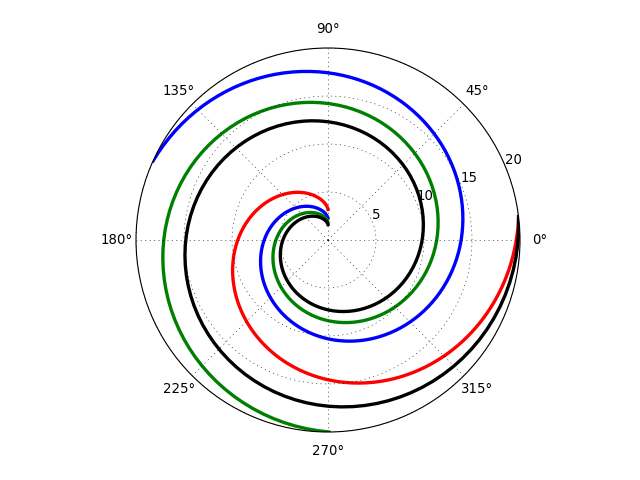
\includegraphics[scale=0.5]{problema4fig1}
 \caption{Superficies de nivel para una partícula libre en coordenadas polares.}
 \label{fig:problema4fig1}
\end{figure}

Si trazamos las perpendiculares a estas curvas vemos entonces que para distintos valores de las constantes estas generarán trayectorias 
de líneas rectas sobre el plano, las cuales son equivalentes a las rectas que deben 
encontrarse para coordenadas cartesianas, solo que estas rectas estarán parametrizadas 
por las coordenadas polares en este caso.

\section{Problema 5}

Utilizando el método de Hamilton-Jacobi reduzca a cuadraturas el péndulo simple. 

\vspace{.3cm}

\underline{Solución:} \vspace{.3cm}

En la figura de abajo se muestra una ilustración del péndulo simple

\begin{figure}[H]
 \center 
 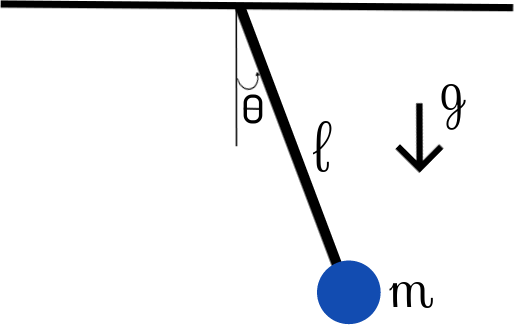
\includegraphics[scale=0.4]{problema5fig1}
 \caption{Péndulo simple.}
 \label{fig:problema5fig1}
\end{figure}

Recordemos que su lagrangiana es 

\begin{equation}
 L = \frac{1}{2}ml^2\dot{\theta}^2 + mgl\cos{\theta},
\end{equation}

el momento $p_\theta$ conjugado a $\theta$ es 

\begin{equation}
 p_\theta = \frac{\partial L}{\partial \dot{\theta}} = ml^2\dot{\theta},
\end{equation}

y por lo tanto la cantidad de Jacobi del sistema es 

\begin{equation}
 H = p_\theta \dot{\theta} - L = \frac{1}{2}ml^2\dot{\theta}^2 - mgl\cos{\theta},
\end{equation}

ahora para escribir la hamiltoniana del sistema escribimos la cantidad de Jacobi 
en términos de $\theta$ y $p_\theta$, 

\begin{equation}
 H = \frac{p_\theta^2}{2ml^2} - mgl\cos{\theta}.
\end{equation}

Claramente la hamiltoniana es igual a la energía total del sistema debido a que 
la lagrangiana no depende del tiempo y la energía cinética es una función cuadrática 
de las velocidades. Ahora podemos escribir la ecuación de Hamilton-Jacobi como 

\begin{equation}
 \frac{1}{2ml^2} \left(\frac{\partial G}{\partial \theta} \right)^2 - mgl\cos{\theta} 
 = - \frac{\partial G}{\partial t}
 \label{eq:HJpendulo1}
\end{equation}

Proponemos una solución de la forma 

\begin{equation}
 G(\theta,t) = W(\theta) + T(t),
\end{equation}

y entonces la ecuación \eqref{eq:HJpendulo1} queda como 

\begin{equation}
  \frac{1}{2ml^2} \left(\frac{\partial W}{\partial \theta} \right)^2 - mgl\cos{\theta} 
 = - \frac{\partial T}{\partial t}.
 \label{eq:HJpendulo2}
\end{equation}

Debido a que el lado izquierdo de \eqref{eq:HJpendulo2} depende únicamente de $\theta$ 
y el derecho de $t$, el único  modo de que esta expresión se cumpla es que ambos
términos sean iguales a una misma constante que llamaremos $\alpha_1$. Entonces 

\begin{equation}
 \frac{1}{2ml^2} \left(\frac{\partial W}{\partial \theta} \right)^2 - mgl\cos{\theta} = 
 \alpha_1,
 \label{eq:HJpendulo3}
\end{equation}

\begin{equation}
 \frac{\partial T}{\partial t} = - \alpha_1,
\end{equation}

de la segunda ecuación vemos directamente que 

\begin{equation}
 \boxed{T(t) = - \alpha_1t.}
\end{equation}

Si utilizamos la definición de $p_\theta$ podemos reescribir \eqref{eq:HJpendulo3} 
como 

\begin{equation}
 \frac{p_\theta^2}{2ml^2} - mgl\cos{\theta} = 
 \alpha_1,
\end{equation}

y entonces podemos asociar a $\alpha_1$ con la energía total del sistema $E$. Volviendo 
a \eqref{eq:HJpendulo3} podemos despejar de ella $\partial W/\partial \theta$ para 
encontrar 

\begin{equation}
 \frac{\partial W}{\partial \theta} = \sqrt{2ml^2(E + mgl\cos{\theta})},
\end{equation}

y por lo tanto 

\begin{equation}
 \boxed{W(\theta) = \int \sqrt{2ml^2(E + mgl\cos{\theta})} d\theta.}
\end{equation}

Y entonces 

\begin{equation}
 \boxed{G(\theta,t) = \sqrt{2ml^2(E + mgl\cos{\theta})} d\theta - Et.}
\end{equation}

Por último calculemos $\beta$, 

\begin{equation}
 \boxed{\beta = \frac{\partial G}{\partial \alpha_1} = \frac{\partial G}{E} = 
 - t + ml^2 \int \frac{d\theta}{\sqrt{2ml^2(E + mgl\cos{\theta})}}.}
\end{equation}

\vspace{.2cm}

con lo cual hemos reducido el problema del péndulo simple a cuadraturas.

\begin{thebibliography}{10}
\bibitem{arfken}
G. Arfken y H. Weber, \emph{Mathematical Methods for Physicists}, 6ta edición, Elsevier 
Academic Press, 2005.
\end{thebibliography}


\end{document}